\paragraph{Functiedefinitie}

Bij functies onderscheiden we de \emph{definitie}, waarin wordt beschreven wat de functie moet doen, van de \emph{aanroep}, die vertelt dat de functie daadwerkelijk moet worden uitgevoerd. Dat betekent meteen dat als we een functie defini\"eren de functie niet direct wordt uitgevoerd. Een functiedefinitie ziet er in dit boek als volgt uit:

\begin{verbatim}
<type> <naam van functie>():
  <inhoud van functie>
\end{verbatim}

Voorlopig zullen we \texttt{void} invullen als \texttt{<type>}. In de praktijk is dat een functie die een opdracht uitvoert (zoals \texttt{print}). Een voorbeeld van een functie die iets doet:

\begin{verbatim}
void ding_printer():
  print("iets")
\end{verbatim}

\paragraph{Functieaanroep}

Van zichzelf doet een definitie niet anders dan een functie defini\"eren onder een gestelde naam. Het aanroepen van de functie gebeurt dan als volgt:

\begin{verbatim}
<naam van functie>()
\end{verbatim}

\paragraph{Traceren} Functieaanroepen kun je traceren. We starten bij de allereerste regel die geen functiedefinitie is, maar een aanroep, en van daar stappen we naar de functie die wordt aangeroepen. Om duidelijk te maken welke functies er zijn, hebben we de definities gemarkeerd met een streep in de kantlijn:

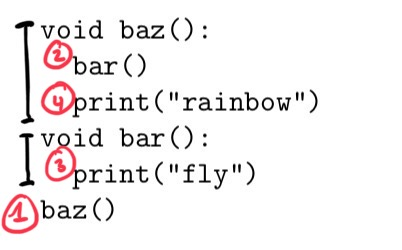
\includegraphics[width=.4\textwidth]{1-trace-calls.jpeg}

Zo zie je in welke volgorde de twee \texttt{print}-statements worden uitgevoerd.
